\section{Rectangle-based Symmetry Reduction}
\label{rooms-based symmetry reduction}

\begin{figure}[]
       \begin{center}
                       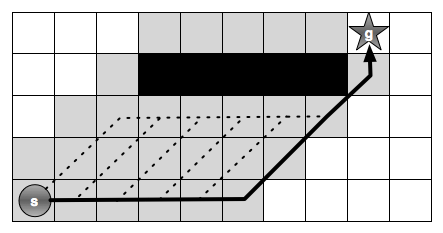
\includegraphics[scale=0.36]{diagrams/symmetry_example.png}
       \end{center}
       \caption{A pathfinding instance with high symmetry. We highlight the
eventual solution returned by A* (strong line) and a number of symmetric 
alternatives (dashed lines).}
       \label{fig-symmetry}
		\vspace{-0.5em}
\end{figure}
%Symmetry is generally regarded as an undesirable characteristic in a search
%space.
There are very few works that explicitly identify and deal with the 
problem of symmetry in a pathfinding context. To address this, we begin by first
making precise the notion of a symmetric relationship between paths:
\begin{definition}
Two paths $\pi_{1}$ and $\pi_{2}$ are symmetric if they share the same start and
goal node and one can be derived from the other by interchanging the order of the
moves.
\end{definition}

See, for example, the pathfinding instance illustrated in Figure \ref{fig-symmetry}.
There are many symmetrical paths, some of which are marked in the figure.
With the popular Octile heuristic in use,
most nodes along symmetrical optimal paths have an $f$ 
value smaller than the $f$ value of the goal. 
Running A* on the original grid will needlessly expand all such nodes.

We will employ the following high-level strategy to
identify and eliminate path symmetries from 4 and 8-connected uniform cost grid maps:
\input alg_rsr

As indicated in the introduction, our approach has similarities with the one used by 
\citeauthor{harabor10}~\shortcite{harabor10}.
Some of the main differences include:
We extend Step \ref{alg:rsr:2} of Algorithm \ref{alg:rsr} 
to include pruning of nodes from the perimeter of an empty room.
We extend Steps \ref{alg:rsr:3} and \ref{alg:rsr:4} of Algorithm
\ref{alg:rsr} in order to facilitate optimal room traversal in 8-connected grid
maps. 
{We introduce a new online pruning strategy that allows faster node
expansion and further speeds up search.}
%The first and the third enhancements work for both 4-connected and 8-connected grids.
%As we will see, the first enhancement can significantly reduce the number of nodes
%in the search space and results in a considerable speedup when compared to 4ERR.

The generalisation to 8-connected grids is more challenging than it might look at a first glance.
On a 4-connected map no tile requires more than one macro-edge
(to the closest tile on the opposite side of the perimeter)
to retain optimality~\cite{harabor10}.
Thus, it is easy to maintain a branching factor on 4-connected maps.
As we show in the next section, many more macro-edges are needed to preserve optimality
on 8-connected maps. We will identify a set of macro-edges that is necessary and sufficient
to ensure that empty rectangles can be crossed optimally.
Keeping the branching factor within reasonable limits
is a primary motivation for the enhancements reported in the next sections.

%\par
%Both speedup enhancements, which we discuss in an upcoming section,
%are applicable to 4 and 8-connected grid maps and both preserve optimality
%during search.
%We term the resultant algorithm \emph{Rooms-based Symmetry Reduction} 
%(or RSR for short).
%\newline \\
%\textbf{Symmetry Reduction in 8-connected Grid Maps:}
%Consider a path which enters an empty room $R$ at some perimeter node $m$ and exits at some other
%node $n$ located on the opposite side of the room.
%On a 4-connected map we can optimally traverse the room by expanding $m$, following
%its macro edge to a node $m'$ on the opposite side of $R$ and finally navigating from $m'$ to $n$.
%The length of this path is equal to the Manhattan distance between $m$ and $n$ and thus optimal.
%However, if the map consists of 8-connected tiles this strategy is no longer optimal.
%In particular, the original (unmodified) map may contain a more direct path to $n$ using one or more diagonal
%transtions.
%\par
%We address this problem as follows:
%First, we give an offline procedure which adds to $R$ a set of additional macro edges
%to facilitate optimal travel between arbitrary pairs of tiles on the perimeter.
%Second, we give an online re-insertion procedure which deals with cases where the start or
%goal is a tile that has been previously removed.
%Finally, we show that this method preserves optimality.
